\documentclass[../main.tex]{subfiles}


\begin{document}

\chapter{Implementation}
\label{chap:implementation}

This chapter describes the libraries that were developed in the scope of this thesis.
They are available in the programming languages Typescript, Python and Go.
This ensures that software components in different environments can handle logs as specified by the protocol.
Details about this practical realization of the libraries can be found in section \ref{sec:implemented-libraries}.
Moreover, the chosen approach heavily influences the existing toolchain.
The existing source code of the toolchain was therefore refactored and adjusted to handle encrypted logs.
This is described in section \ref{sec:toolchain-modifications}.

\section{Implemented Libraries}
\label{sec:implemented-libraries}

The following table gives an overview of the implemented libraries.
It includes links to the GitHub repositories and the package indexes of the programming languages where the libraries were published.
The acronym \emph{it-crypto} stands for inverse transparency cryptography.

\begin{table}[ht]
    \centering
    \begin{tabular}{|c|c|c|c|}
    \hline
    Name         & Language & Github                           & Link to package index                                   \\ \hline
    Ts-it-crypto & Typescript           & \href{https://github.com/haggj/ts-it-crypto}{haggj/ts-it-crypto} & \href{https://www.npmjs.com/package/ts-it-crypto}{NPM}       \\ \hline
    Py-it-crypto & Python               & \href{https://github.com/haggj/py-it-crypto}{haggj/py-it-crypto} & \href{https://pypi.org/project/py-it-crypto/}{PyPI}          \\ \hline
    Go-it-crypto & Go                   & \href{https://github.com/haggj/go-it-crypto}{haggj/go-it-crypto} & \href{https://pkg.go.dev/github.com/haggj/go-it-crypto}{PKG} \\ \hline
    \end{tabular}
    \caption[Overview implemented libraries]{Overview and links of the implemented libraries to handle encrypted logs.}
\end{table}

All three libraries are fully tested and compatible with each other.
Data that was encrypted in one library can be decrypted by all libraries.
It was taken care that classes, functions, constants, and variables are named similarly (identical names are not possible because of the different naming conventions in Go, Python and Typescript).
Moreover, all libraries employ the same folder structure.
This aims to improve the maintainability of the source code.
As a result, all three libraries expose the same interface to users.
This interface is highly related to the algorithms described in chapter~\ref{chap:design}.
The designed protocol relies on the JOSE standard.
Thus, each library depends on a third-party package implementing JOSE.
Ts-it-crypto depends on the Typescript package JOSE\footnote{\url{https://www.npmjs.com/package/jose}}.
Py-it-crypto depends on the Python package \emph{jwcrypto}\footnote{\url{https://pypi.org/project/jwcrypto/}}.
Go-it-crypto depends on the Go package JOSE\footnote{\url{https://pkg.go.dev/gopkg.in/square/go-jose.v2}}.

\subsection{General usage}

This section describes the usage of the implemented libraries in general.
Please also refer to the pseudocode depicted in listing~\ref{lst:pseudocode}.
If you are interested in the concrete realization in a specific language have a look at the corresponding Github repositories.

To make use of the library an instance of type \verb|ItCrypto| must be instantiated.
This instantiation requires the function \verb|fetchUser|.
It resolves an identity of a user (which is a \verb|string|) to an instance of type \verb|RemoteUser|.
The function usually requests a server resolving the identity of a user to its public keys.
It needs to implement the following signature: \verb|RemoteUser fetchUser(string)|.
A \verb|RemoteUser| object stores the public keys of the user along with its identity and the information if the user is a trusted monitor.
This information is mainly used during decryption to verify if the signed data is valid.
Please note that a \verb|RemoteUser| object should never be constructed directly.
Rather, the \verb|importRemoteUser| function must be called.
This function expects a trusted certificate as a parameter.
This trusted certificate is assumed to contain the public key of a root certificate authority within the PKI.
The public keys of all users are assumed to be signed by this certificate authority.
The function \verb|importRemoteUser| verifies if the provided public keys are signed accordingly.

Once the \verb|ItCrypto| object is instantiated a user needs to log in.
A logged-in in user is represented by an \verb|AuthenticatedUser| object.
It extends the \verb|RemoteUser| object because it additionally provides the private keys of the user.
This allows the logged-in user to sign and decrypt data.
A login is realized by calling the \verb|login| method on the \verb|ItCrypto| object.
This function expects the PEM-encoded key material.
If a user is logged in the \verb|ItCrypto| object becomes fully functional.
The logged-in user can create, encrypt and decrypt logs using the provided keys.

\definecolor{codegreen}{rgb}{0,0.6,0}
\begin{lstlisting}[basicstyle=\small, label=lst:pseudocode,float,floatplacement=tbp, language=Java, caption={[Pseudocode library usage]Pseudocode of creating, encrypting and decrypting logs using the provided libraries.}, morekeywords={RemoteUser, var, assert}, commentstyle=\color{codegreen}]
RemoteUser fetchUser(string identity){
    /*
    Fetch keys from the server and check if a user 
    is a trusted monitor.
    */
    return importRemoteUser(
        identity,
        /* keys */, 
        isMonitor, 
        rootCA
    )
}

// Initialize itCrypto object
var itCrypto = ItCrypto(fetchUser)
itCrypto.login(/* keys */)

// Sign log data
var signedLog = itCrypto.signLog(/* log data */)

// Encrypt log for a set of recipients
var alice = fetchUser("identity@alice.com")
var bob = fetchUser("identity@bob.com")
var loggedInUser = itCrypto.user
var encryptedLog = itCrypto.encryptLog(
    signedLog, 
    [alice, bob, loggedInUser]
)

// Decrypt log
var decryptedLog = itCrypto.decryptLog(encryptedLog)
assert(decryptedLog == signedLog)
\end{lstlisting}

\subsection{Documentation ItCrypto}
This section further details the \verb|ItCrypto| object.
It aims to provide documentation for developers who integrate the library into their software.
In particular, the methods \verb|signLog|, \verb|encryptLog| and \verb|decryptLog| are detailed.
As described in chapter~\ref{chap:design}, those methods can be used to provide the full functionality of the intended protocol.

The method \verb|signLog| cryptographically signs the given log data.
Monitors must call this encryption function to initially sign an instantiated log.
The protocol does not allow any raw logs in the system.
Rather, all logs must be signed by the monitor that created the log. 
This method relies on the private signing key of the logged-in user.
\begin{table}[ht]
    \centering
    \begin{tabular}{|p{3cm}p{10cm}|}
        \hline
        \multicolumn{2}{|l|}{Input parameters}    \\ \hline
        \verb|accessData|              & This is a data structure containing the raw log data. In particular, this raw data must be encodable as JSON data. It contains all relevant information to log the observed data access.           \\ \hline
        \multicolumn{2}{|l|}{Output}   \\ \hline
        \multicolumn{2}{|p{13cm}|}{The method returns a JWS token encoded as string. It is signed by the logged-in user and it contains the JSON-encoded accessLog as payload.} \\ \hline
    \end{tabular} 
    \caption[Signature of signLog]{Input parameters and output of the signLog method.}
\end{table}

The method \verb|encryptLog| encrypts a given log for a given set of recipients.
Monitors must call this function to initially encrypt the log for the data owner.
It is crucial to the security of the protocol that the monitor only chooses the data owner as a recipient. 
This encryption function can be used to share or revoke access to the log.
In this case, it must be called by the data owner of the particular log. 
This method relies on the private signing key of the logged-in user.
\begin{table}[ht]
    \centering
    \begin{tabular}{|p{3cm}p{10cm}|}
        \hline
        \multicolumn{2}{|l|}{Input parameters}    \\ \hline
        \verb|log|              & This is the log that needs to be encrypted. It must be signed by a monitor. The output of \verb|signLog| can be directly used here.           \\
        \verb|recipients|       & This is a list of \verb|RemoteUser| objects containing the identity and public encryption key for each recipient. This set defines which users can decrypt the created cipher.           \\ \hline
        \multicolumn{2}{|l|}{Output}   \\ \hline
        \multicolumn{2}{|p{13cm}|}{The method returns a JWE token encoded as string. It contains the provided signed log and can only be decrypted by the specified recipients. The token specifies the logged-in user as creator of the token. It also contains the set of recipients and the identity of the data owner as metadata.} \\ \hline
    \end{tabular}
    \caption[Signature of encryptLog]{Input parameters and output of the encryptLog method.}
\end{table}

The method \verb|decryptLog| decrypts a given encrypted data.
A user can only decrypt this log if it was included as a recipient during encryption.
It might be called by any user that received an encrypted log.
The method performs multiple validations to detect any misusage of the protocol.
In particular, it verifies all signatures of the encoded JWS tokens.
This function relies on the private decryption key of the logged-in user.
\begin{table}[ht]
    \centering
    \begin{tabular}{|p{3cm}p{10cm}|}
        \hline
        \multicolumn{2}{|l|}{Input parameters}    \\ \hline
        \verb|jwe|              & This is a JWE token that represents an encrypted log. This token is the result of \verb|encryptLog|. \\ \hline
            \multicolumn{2}{|l|}{Output}   \\ \hline
        \multicolumn{2}{|p{13cm}|}{The method returns a log. This is the same object that was passed to the encryption function. Therefore it is still signed by a monitor. The signature, however, was already verified during decryption. This construction allows a data owner to easily re-encrypt the log.} \\ \hline
    \end{tabular}
    \caption[Signature of decryptLog]{Input parameters and output of the decryptLog method.}
\end{table}

\subsection{Cryptographic keys}
The libraries require cryptographic keys to create, encrypt and decrypt logs.
As described in section~\ref{sec:overview}, the protocol assumes an externally established PKI.
Each user is assigned two key pairs (one for signing and one for encrypting data).
The private keys are assumed to be PEM-encoded.
Public keys are assumed to be PEM-encoded certificates that are signed by a trusted certificate authority.
Whenever a user is imported, the certificates of the user are assumed to be signed by this certificate authority.
Currently, the libraries only support elliptic curve cryptography.
The elliptic curve OpenSSL parameters \verb|prime256v1| are known to work in all three implementations.

\section{Toolchain modifications}
\label{sec:toolchain-modifications}
The integration of the protocol requires the adoption of the existing toolchain.
Figure~\ref{fig:encrypted-toolchain} was taken from~\cite{Zieglmeier2021}.
It additionally visualizes the encrypted data flow in the toolchain.
In particular, a monitor encrypts the log for the data owner.
A user who is logged in to the display component can decrypt its logs.
Moreover, access to the logs can be shared and revoked.
This functionality requires changes in the \emph{Monitor}, \emph{Safekeeper} and \emph{Display} component.
Those changes were implemented in the context of this thesis.
The development environment of the toolchain is a proof-of-concept.
It shows how a \emph{PKI} infrastructure can be used to integrate encrypted logs.
The following sections describe different perspectives on this integration.
They provide details about the implemented changes.


\begin{figure}[h!]
    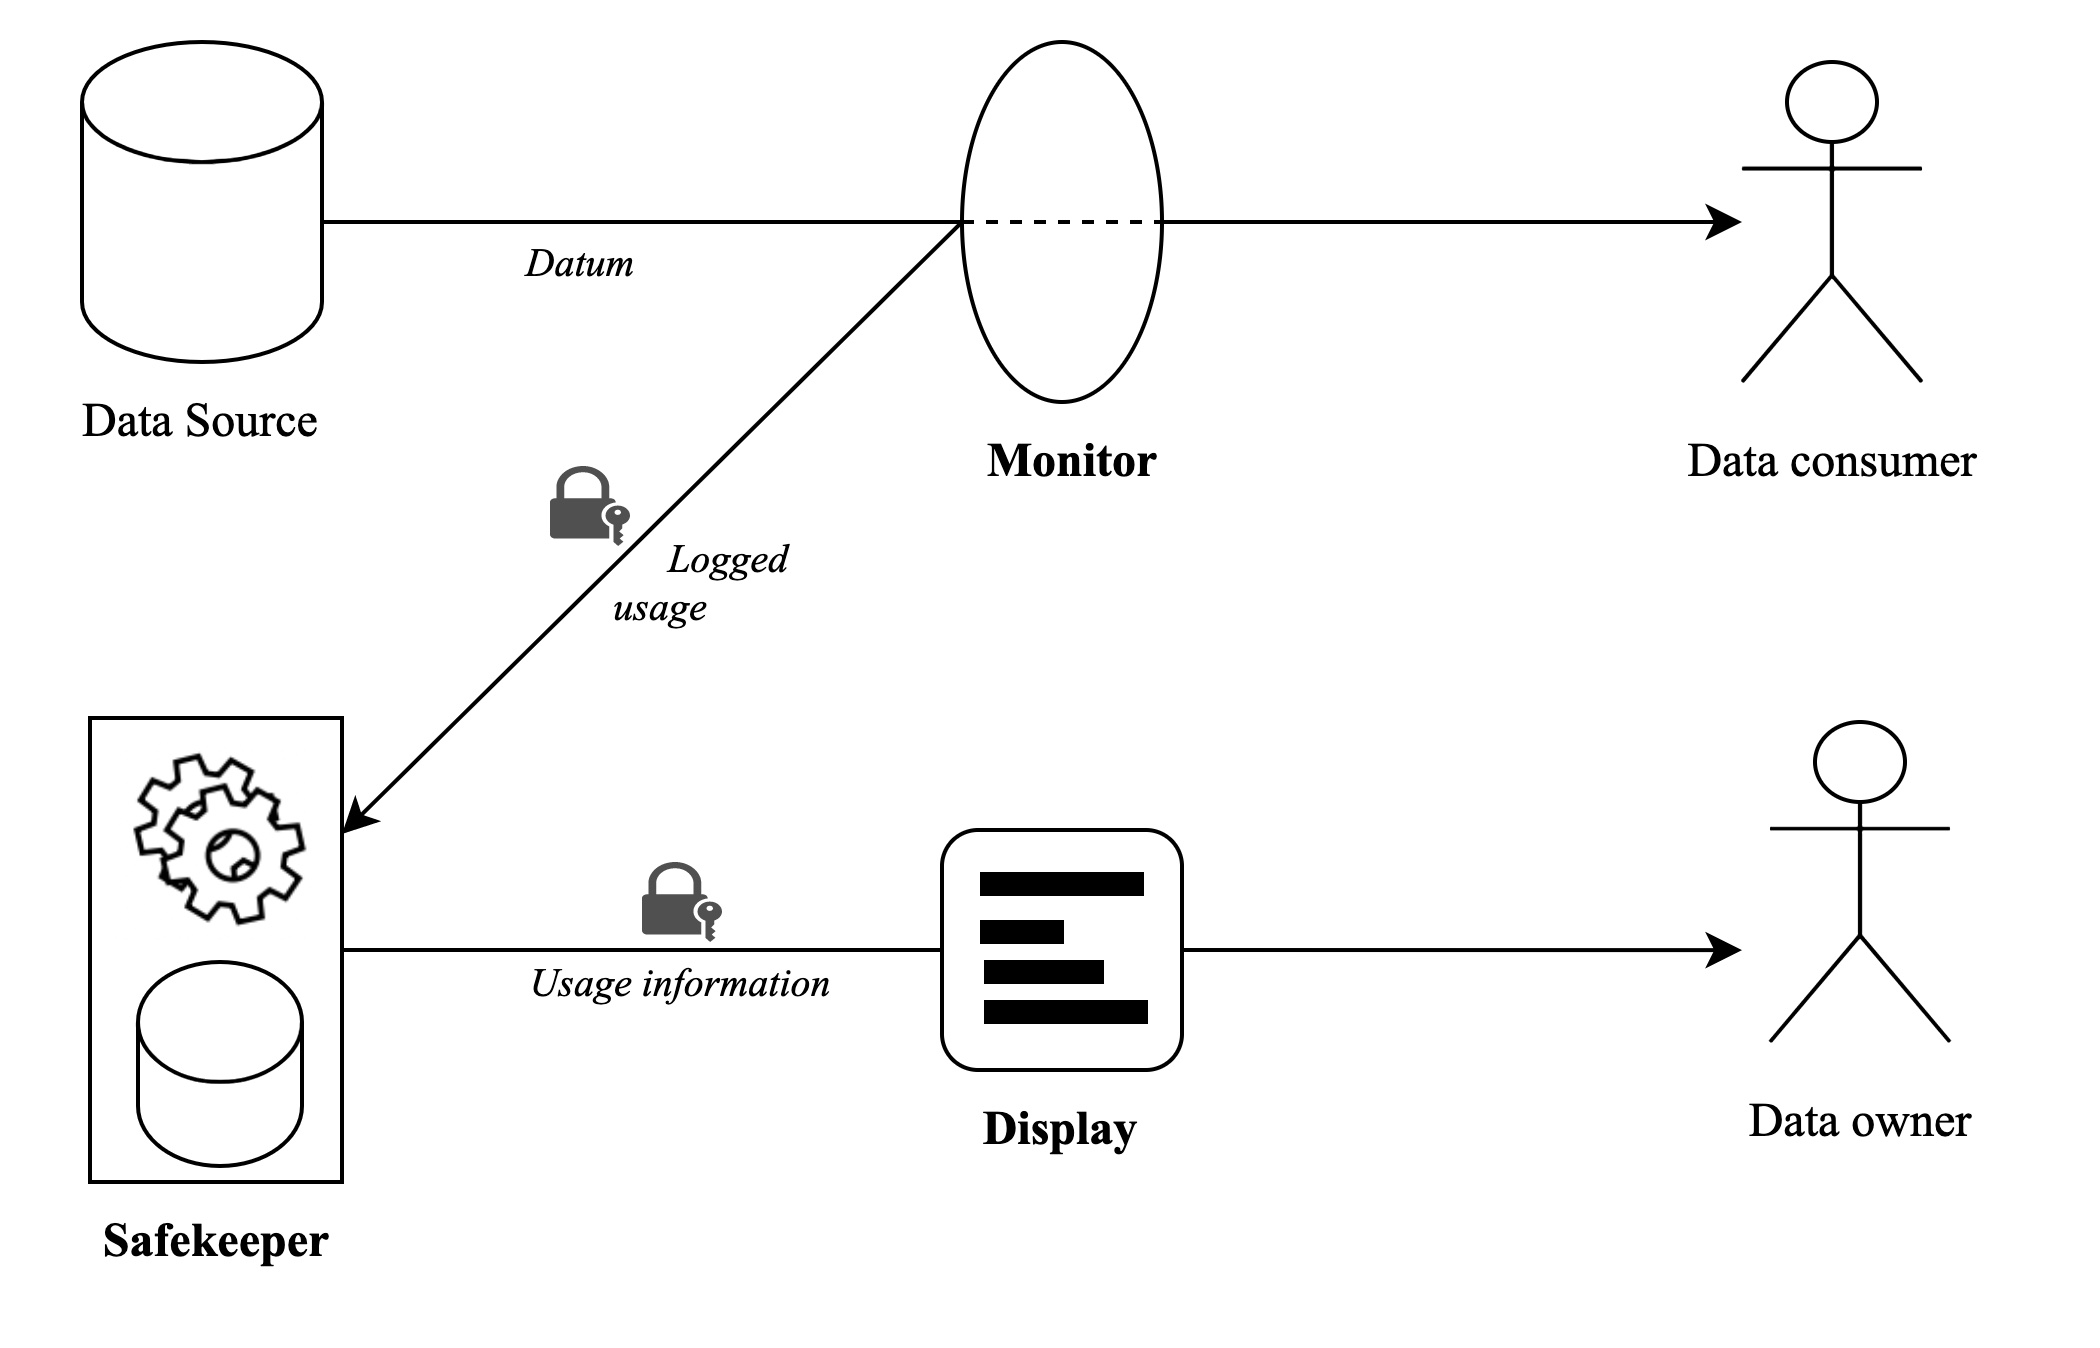
\includegraphics[width=8cm]{../img/06/encrypted_toolchain.jpg}
    \centering
    \caption[Toolchain encrypted data flow]{The general data flow in the toolchain has not changed. The passed data, however, is end-to-end encrypted.}
    \label{fig:encrypted-toolchain}
\end{figure}

\subsection{User management}
The toolchain relies on a single-sign-on server responsible for authenticating users.
The development environment provides the \emph{Revolori} server which is an implementation of this service.
Besides the user information it now additionally stores certificates containing the public keys of the users and the information if a user is an authorized monitor.
This additional information is used by the front-end to encrypt and decrypt logs.
Therefore, a new endpoint was introduced which resolves the identity of this information (e.g. the certificates and if the user is a trusted monitor).

The development environment of the toolchain is a proof-of-concept that shows how an external PKI can be connected.
There are two scripts used to load pre-configured users into the development environment.
Both were updated to establish an exemplary PKI:

\begin{itemize}
    \item 
    The script \verb|prebuild.sh| is responsible for creating a key pair for the \emph{Revolori} server.
    It is used to sign access tokens.
    The public key is passed to the \emph{Overseer} because it needs to verify if a provided token was signed by the \emph{Revolori} single-sign-on-server.
    
    The script was adopted to create a key pair for an exemplary certificate authority.
    Moreover, the script expects a file \verb|users.json| which contains the pre-configured user data.
    Two key pairs for each user are generated.
    The public keys of all users are signed by the public key of the certificate authority.
    This effectively creates certificates binding the identities of the users to their public keys.
    Finally, the script updates the provided \verb|users.json| to contain the cryptographic keys of each user.
    \item 
    The script \verb|setup.sh| is responsible for creating users in a running \emph{Revolori} instance.
    It is also used to create exemplary data accesses for each user.
    Thus, the script had to be adopted to support encrypted logs.
    First of all, the script expects the file \verb|users.json| which contains user information along with their cryptographic keys.
    It then parses the user information and creates the respective users in the \emph{Revolori} server.
    In particular, this includes the certificates of the user's public keys.
    To pre-compute encrypted logs the \emph{CLI} of the \emph{ts-it-crypto} library needs to be installed.
    It allows encrypting log data in the name of a monitor.
    The encrypted logs are then uploaded to the \emph{Overseer}.

\end{itemize}

This setup allows fetching the public keys for a given user from the \emph{Revolori} server.
The development environment also provides the private keys for a user upon login.
This is realized by passing the \verb|users.json| file to the \emph{Clotilde} process.
Please note that this implies that the front-end has unrestricted access to all private keys.
Thus, this setup can only be used in the development environment.
In productive systems, the \emph{Clotilde} front-end must securely import the private keys from the user (e.g. via hardware token).
If a user logs in to the system, the front-end instantiates an \verb|ItCrypto| object using the provided key material.
This finally enables all cryptographic tasks.


\subsection{Display component}
The display component is the front-end of the toolchain.
It visualizes all data accesses concerning the logged-in user.
Since all logs are end-to-end encrypted it must handle the logs provided by the \emph{Safekeeper}.
In particular, the logs must be decrypted in the front-end.
Access to the logs can also be shared and revoked by the data owner.
This allows a data owner to authorize any other user in the system to temporarily access a log.
The adopted implementation provides this functionality.
To perform the necessary cryptographic actions, it integrates the \emph{ts-it-crypto} library into the front-end application.
Appendix~\ref{app:screenshots} contains screenshots of the realized UI.

\subsection{Safekeeper component}
The \emph{Safekeeper} component is responsible to store logs.
It was adopted to handle encrypted data.
As described in section~\ref{sec:metadata}, an encrypted log contains metadata to support intermediate servers.
This metadata contains the set of recipients (e.g. the users that can decrypt the log) and the identity of the data owner.
Once a loc is sent to the server, thus, this metadata must be parsed.
It is stored along with the encrypted log in the database.
This allows the \emph{Safekeeper} to associate a log with users.
A new endpoint was implemented that allows users to request its encrypted logs.
Based on the provided metadata, the server can filter all logs concerning this particular user.
Moreover, the data owner of a log can update a log to share or revoke access.
Thus, a second endpoint was created that allows data owners to modify stored logs.

Since all logs are end-to-end encrypted it can not access any content of the stored data.
This implies that it can not verify if a performed access was permitted by the data owner.
However, those endpoints still exist.
This allows data owners to provide detailed policies about who can access what data.
A monitor tracking data usage and creating corresponding logs can check if the observed access is allowed by calling those endpoints.
Since the \emph{Safekeeper} can not validate the compliance of these policies, this validation is outsourced to the monitor.



\end{document}
